%!TEX root = main.tex

\section{Study Results}

%!TEX root = ../main.tex

\begin{table*}
\caption{Programming activities and the most frequently accessed artifacts associated with them}
\label{tab:programming-activities}
\begin{tabular}{lll}
\toprule
Programming Activity & Artifact type [frequency] & Artifact type frequencies for each type \\
\midrule
\multirow{3}{*}{A0 - Coding} & Code [32] & [2,6,5,4,12,2,1] \\
& Tools [12] & [1, 1,5,1,3,1] \\
& Documents [2] & [2] \\
\midrule
\multirow{2}{*}{A1 - Interaction with documents} & Documents [19] & [19] \\
& External Artifacts [20] & [13,7] \\
\midrule
\multirow{2}{*}{A2 - Navigation} & Code [9] & [0,1,1,0,5,1,1] \\
& Tool [1] & [0,0,1,0,0,0] \\
\midrule
\multirow{2}{*}{A4 - Reading Task Prompt} & Documents [22] & [22] \\
& External Artifacts [15] & [10,5] \\
\midrule
\multirow{2}{*}{A5 - Searching in web/IDE} & Code [4] & [0,0,1,1,2,0,0] \\
& Tool [1] & [0,0,1,0,0,0] \\
\midrule
\multirow{2}{*}{A6 - Reading Search Results} & Code [1] & [0,0,0,0,1,0,0] \\
& Web Resource & [1] \\
\midrule
\multirow{2}{*}{A7 - Processing Search Results} & Code [2] & [0,0,0,0,2,0,0] \\
& Web Resource & [1] \\
\midrule
\multirow{2}{*}{A8 - Viewing Web Resource} & Code [1] & [0,0,0,0,1,0,0] \\
& Web Resource & [1] \\
\midrule
A9 - Debugging & Code [1] & [0,0,0,0,1,0,0] \\
\midrule
\multirow{2}{*}{A11 - Idle} & Documents [2] & [2] \\
& External Artifacts & [1,1] \\
\bottomrule
\end{tabular}
\end{table*}

\begin{figure}
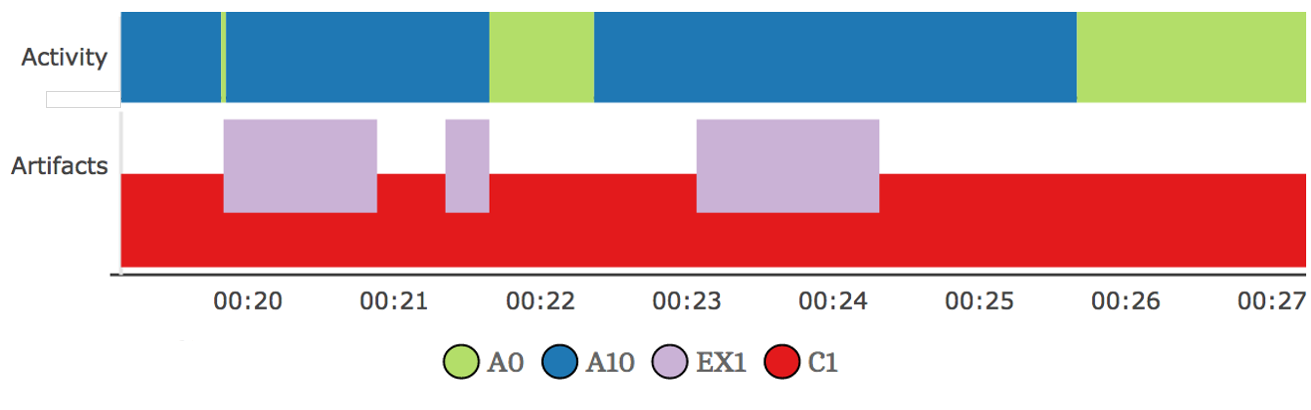
\includegraphics[width=\columnwidth]{figures/P1timeplot}
\caption{Time sequence of Activities and Artifacts from P1}
\label{P1Fig}
\end{figure}

\boldification{here we report on how participants created and used context as they were working on their programming task.}
Here we present our observations of how participants' interact with the artifacts during specific programming activities. Our focus was to develop an understanding of how the context building process occurs, and gain insights into which factors play a role in shaping context.


We observe the types of artifacts that participants refer to when performing different programming activity. The participants interacted with six different types of artifacts: \textit{source code files} (e.g. \texttt{intersection.js} and \texttt{car.java}), \textit{documents} (task prompt), \textit{IDE tools} (\textit{New Class} dialog box, getter-setter dialog boxes (e.g. \texttt{T2}), terminal/console),\textit{ web resources} (e.g. Google search results, Stack-Overflow pages, API documentation), \textit{externalized artifacts} (e.g. sticky notes, paper diagrams), and \textit{other} (e.g. calculators).

For each participant, we refer to source code files in the format \texttt{(C1,C2,\ldots,)}, the prompt document as \texttt{(D1)}, IDE tools as \texttt{(T1,T2,\ldots,)}, web resources as \texttt{(W1,W2,\ldots,)}, and external artifacts as \texttt{(EX1)}. The numbering of these tags represents the sequential order in which participants encountered or interacted with them.
%%% INSERTING FIGURE FOR P4'S ACTIVITIES AND ARTIFACTS HERE.

% We didn't restrict our observation to any medium, as context is a broad notion and anything around a person, from the placement of a paper to the color of the screen, can affect it. We also collected diverse data in the form or think aloud, screen capture, facial expression, video of workspace and any notes or diagrams the participants drew to recognize the subtle hints which may suggest that information was added to the context or obtained from the context. 

%Collecting screen capture, audio, and any notes or diagrams the participants drew, we identified the different types of artifact the participants use. 

%Table~\ref{tab:programming-activities} presents the programming activity that P4 performs and the artifacts she interacts when performing the programming activities. The first column shows all the programming activities that P4 performed, out of the 12 activities discussed in Table~\ref{tab:programming-activities} that we coded. The second column shows the frequency with which P4 accessed each type of artifact within each programming activity. The third column shows a breakdown of the artifacts for each type, with the frequency of each artifact shown as bar graphs. Artifact names have been anonymized for analysis purposes. 
\boldification{**We identify the type of artifact and the specific instance of the artifact correlated with the type of programming activity to get a finer-grained understanding of what was used to create context. Table x...does this.}



%There are 7 code files (which we coded as c1.java, c2.java, \ldots, c7.java) that P4 created and worked with iteratively during the observational session. She used 6 IDE tools (t1, t2,..., t6) and referred to 1 document (d1) during this time. However, she also referred to 2 web sources (coded as w1 and w2) and created two external artifacts on paper (ex1 and ex2) that she repeatedly referred to.

\subsection{Artifacts span heterogeneous medium}
\boldification{**participants used all kinds of artifacts**}
During our study, participants not only accessed code artifacts, but also tools within the IDE, online resources, and external documents to help them in their programming task. Here we discuss the different types of artifacts and the frequency in which they're used.

\boldification{**code was obviously the most}
Participants, as can be expected, accessed the code artifacts most frequently when involved in their coding activity \texttt{(A0)}. During their hour-long session, P1 accessed three source code files 87 times, P4 accessed seven source code files 49 times, and P6 accessed four source code files 147 times. 

\boldification{**next was online resources. P6 used website this way}
The next most frequently accessed artifacts were on-line resources. Participants often used these resources to learn how to use a feature or recall implementation details. For example, P6 accessed seven web resources 91 times---he used blog posts to learn how to correctly use the ``\texttt{draggable}'' feature when he had difficulty implementing the feature. Brandt et. al.~\cite{Brandt:2009}, across two studies, found similar ways in which participants use on-line resources.

\boldification{**people also used external artifacts - designing, enriching. P1 did this. Here is his external artifact pictures}
We found that participants also engaged frequently in creating external artifacts (e.g., notes, updating the traffic prompt, and creating diagrams). Figure~\ref{P1Fig} shows a plot of P1's activities and the artifacts he interacts with for an 8-minute segment of his session. We found that P1 (based on his think aloud data) was ideating about possible solutions. If we simply analyze his on-line interactions it shows that he was interacting with the code file \texttt{intersection.scala (C1)} while his programming activity switched between coding \texttt{(A0)} and being idle \texttt{(A1)}. However, this belies the fact that he was ideating different solutions during this period. More specifically, he was modeling the traffic movement at the intersection (Fig~\ref{P4Sketch}.A) and the data model to represent the  intersections (Fig~\ref{P4Sketch}.B).

\boldification{**This means just looking at artifacts that are within IDE like Gail does leaves big gaps}

Our observations indicate that when defining context and how it is built, we need to also consider artifacts that are outside the IDE. Not doing so, as has been done in the past ~\cite{Gasparic:2017,Kersten:2006}, leaves gaps in our understanding and increases the difficulty in modeling context.

% From the plot, near the 22 minute mark, when P1 interacts with the code artifact c1, he was ideating while thinking aloud. However, his programming activities go from idle [A11] to communicating [A2] to selecting parts of the code as part of thinking aloud (marked as coding [A0]) and back to being idle [A11] in the IDE. 

%Simply analyzing artifacts in the IDE, such as different code files, as the primary source of context as done by the representational view can leave gaps in our understanding.

% looking only at online (especially code) artifacts provide a tiny facet of what makes constitutes the whole process of context building during a programming task. During the interaction with web resources and periods of ideating, participants made progress towards solving the problem which they later implement. These non-IDE sources are factors that affect context, if not being part of the context itself.


%==============================================================
%-------------------- END 4.1 ---------------------------------
%==============================================================

\subsection{Programming activity guides interaction with artifacts}

\boldification{Participants accessed same artifacts for many different purposes (different aspects of programming). We find that the same artifacts were used to create context (understanding a problem, ideate) and apply context to form solution (form solution, code)**. For example?..in table x, we see?.}

Participant's interactions with these different types of artifacts varied based on the type of activity they were performing at the time of the interaction. The programming activity guided the kinds of artifacts, and medium, that were accessed and also how participants interacted with the artifact.

\boldification{**activity guided which artifacts and the interaction with the artifacts. P6 example of code artifact for coding and searching activity}

For example, from Figure~\ref{P6Fig}.A, when interacting with the code artifact \texttt{cards.js (C1)}, P6 was actually involved in two separate activities (coding \texttt{(A0)} and searching \texttt{(A4)}. To update a feature, P6 produces new code in \texttt{cards.js (C1)} but then realizes that he needs to update all the other parts of the program that were affected. He searches for the particular term within the code and switches back to coding as necessary. While both of these activities, coding \texttt{(A0)} and searching \texttt{(A4)}, required P6 to interact with the code artifact \texttt{C1}, the type of interaction varied. When coding \texttt{(A0)} between \texttt{00:15:57} to \texttt{00:16:29}, P6 primarily typed in short bursts that were interspersed with scrolling interactions. Whereas, during searching \texttt{(A4)} from \texttt{00:16:29} to \texttt{00:17:02}, P6 mostly scrolled following the highlighted instances of the term he searched and intermittent copied text.

%-->however, we also observed that the interactions with these artifacts were guided by the activities being performed with the artifacts. For example, P6 in Figure~\ref{P6Fig}.A is observed interacting with a source code file (\texttt{C1}, \textit{Artifacts}) while coding (\texttt{A0}, \textit{Activities}) from 00:15:57 to 00:16:29, but then switches to searching (\texttt{A5}, \textit{Activities}) for all instances of a particular term within the project from 00:16:29 to 00:17:02. Both of these activities occur within the same source code file, but the purpose and interactions are different. When coding (\texttt{A0}, \textit{Activities}) within the source code file, P6 primarily types in short bursts that are interspersed with scrolling interactions. When searching (\texttt{A5}, \textit{Activities}) within the source code file, P6 primarily scrolls with intermittent highlighting and copying of text.

\boldification{**interactions with artifacts guide the activity}
The interactions with artifacts provides the information which guides activity forward, sometimes causing a switch to different activity. In Figure~\ref{P6Fig}.B, P6 looks through a \texttt{stackoverflow.com} page \texttt{(W3)}. He is viewing web resources \texttt{(A7)}, scrolling and intermittently pausing to read the answers on the page until he finds a probable answer. Then he switches to coding \texttt{(A0)}, and for the next two minutes, continued to switch between the coding \texttt{(A0)} and viewing web resources \texttt{(A7)}. Toward the end of this sequence of activities, P6 scrolled quickly to a desired section and copied the text before returning to code.

%P6 searched...got results, that he scrolled through several results, he then looked further into an SO post where he read the post, until he found a probable answer. He then switched to coding and kept switching back and forth to the particular SO answer while coding.

\boldification{**sunset para: both matter}
While the above examples are intuitive and simple, they shed light on how activity and interactions with artifact are closely tied together. They provide evidence to the notion that not only does context arise from the activity, the programming activity and the goal behind it guide the specific type and amount of information obtained from the artifact. And that this combination of factors further delineates the context.

%=========================================================
%---------------------------END 4.2-----------------------
%=========================================================

%\boldification{Participants accessed same artifacts for many different purposes (different aspects of programming). We find that the same artifacts were used to create context (understanding a problem, ideate) and apply context to form solution (form solution, code)**. For example?..in table x, we see?.}

%Across different programming activities, participants access the same artifacts. Figure~\ref{P4Fig} shows the sequence of activities P4 performed and the artifacts she interacted with during a small part of her session. On a timed scale, the top bar shows the activities as time progresses, the bottom bar shows the   

%We scrutinize P4's activities within a smaller window of time.- coding to debugging then navigating between 4 different code files followed shortly by navigation to task prompt to read a highlighted portion -- then finally moving to create a new code file.



%used the code file c5 12 times when she was coding [A0] and nine times when she was navigating. When we look closer, during the 60 minute session, all the navigations to c5 were not all for the purpose of coding. P4 coded [A0] in c5 for some time, moved to the requirements document [A4] and spent some time reading it. P4 briefly moved to c5 from the document, read through her code which we infer as an action to verify if her code meets the her design to meet the requirements. She went back to the requirements document [A4] and finally moved to the c5 file to start coding [A0] again. ---story changed due to difference in timeline ---

%in another instance, P4 moved from coding[A0] in c5 to searching on the web [A5] how to implement a certain concept, reading the search results [A6], choosing one that she perceived to be of highest value [A7] and finally reading the webpage she chose [A8]. She moved back and forth between the webpage w1 and the codefile c5 two times. Both times her cursor was on a part of the web page w1 which was a code snippet -- we inferred that she was checking for syntactical differences or errors. 

%These observations reveal that the same artifacts are used across different programming activities.This contradicts the representational view of context, which suggest that ``context and activities are separable'' \cite{Dourish:2004,Gasparic:2017}. We see a difference in the type of artifacts across activities. Programming activity is an important aspect to consider when determining context. 



% \subsection{Programming activity guides interaction with artifacts}

\begin{figure*}
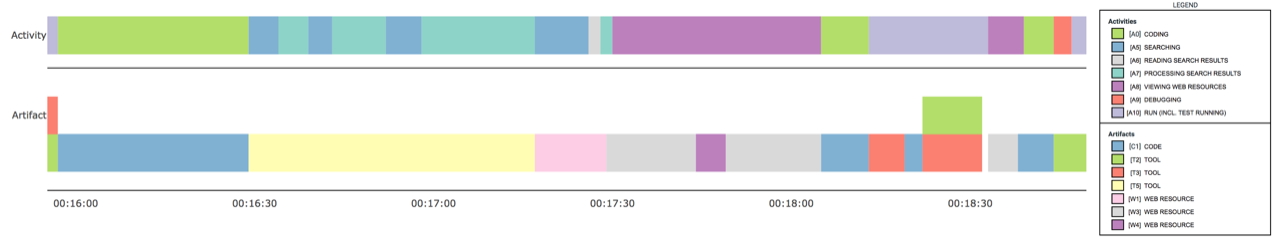
\includegraphics[width=2.05\columnwidth]{figures/P6timeplot}
\caption{Time sequence of Activities and Artifacts from P6 during study; \protect\circled{A} shows a sequence of \texttt{CODING (A0)} and \texttt{SEARCHING (A4)} across the same \texttt{C1} source code file, \protect\circled{B} represents a cycle of evaluation, action, and reflection.}
\label{P6Fig}
\end{figure*}


% \begin{figure}
% 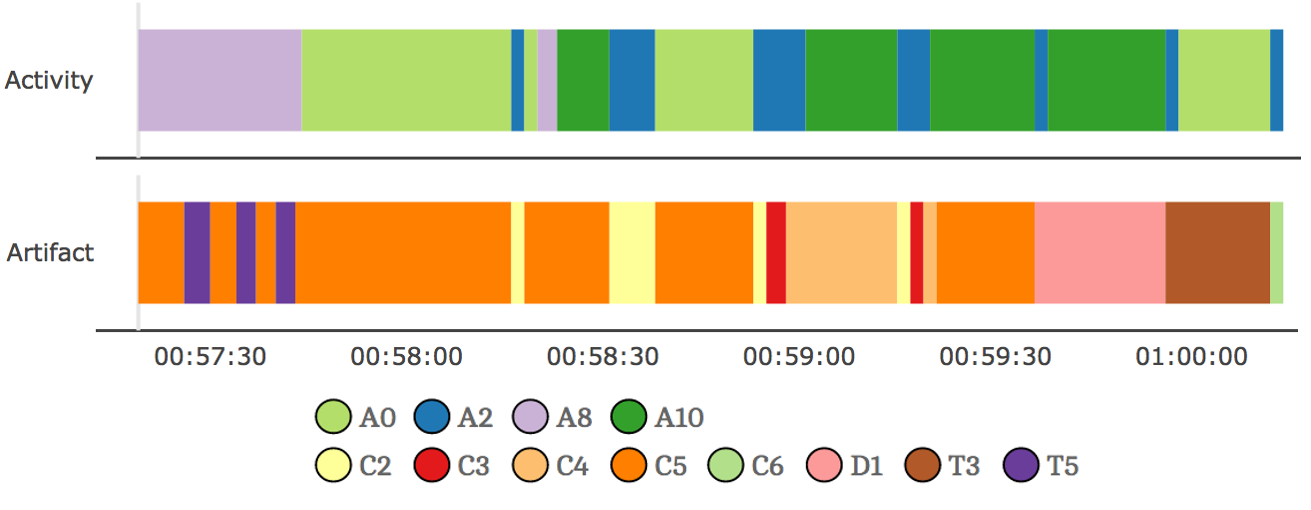
\includegraphics[width=\columnwidth]{figures/P4timeplot}
% \caption{Snippet of Activities and Artifacts from P4 (traffic intersection prompt, 3-minute duration)}
% \label{P4Fig}
% \end{figure}
% \boldification{**based on the activity, the interaction with artifacts change**}

% When participants access the artifacts, the specific interactions with the artifacts -- selecting which part of the artifact to go to, whether they simply scroll through the artifact or highlight parts of the artifact, whether they copy text from these artifacts to paste into the code for debugging -- depends on the programming activity and the goal driving the activity. These differences are also observable through the difference in times spent on these artifacts.

% Figure~\ref{P6Fig} shows the artifacts P6 accesses and the activities he performs. A marks the time P6 searched on the web to obtain the syntax for a java script feature. The first time he reaches a Q and A web page containing answers to his question (marked B) on the diagram, he scrolls through the first few answers before selecting one spending around 36 seconds. These interactions was driven by the goal to learn how to implement the feature for the purpose of coding [A0]. When his selected answer threw an error (marked as C), he went back to the web page and quickly scrolled and found the answer he had already identified (marked as D) and copies it to implement. This second visit to the web page took only five seconds and was geared towards recalling the syntax for debugging purposes [A9]. 

% Brandt et. al.~\cite{Brandt:2009} observed similar behavior in programmers where he was able to distinguish between the purposes of when programmers use online resources. He also found that participants spent the most time when learning from the web and least time when using the web to recall syntax.

% \boldification{**memory plays a role - sequence matters [same activity, shorter time, memory plays role] [zoomed out figure]}

% We also observe that memory plays a role in the interaction with artifacts. In the above example, across the different the coding [A0] and debugging [A9] activities, when P6 visited the web page a second time it took him exactly five seconds to locate the syntax and copy it. We infer that he could recall from his memory where the desired information was located. We observe such a mapping between information and artifacts were referred to by the participants repeatedly. This mapping was influenced by the programming activities and the goal behind the activities.

% \boldification{**Not only does context rise from the activity i.e. activity guides the specific type and amount of information obtained from the context/artifact, the activity was used to recall the relation between the context with which the artifacts were associated**}

% Thus, we see that not only does context rise from the activity, the programming activity and the goal behind it guides the specific type and amount of information obtained from the artifact that comprises the context. The programming activity is used to recall the relation between the information and the artifacts within the context.


% \boldification{**this means that?.and is contrary to the assumptions of ?representational view of context, that context is stable and separate from activities? [...], is not what we see in our data. }

\subsection{Interaction includes Reflection}

\boldification{**Finally we see that, users conduct reflection/evaluation of the information they come across before deciding their next activity**}

Participants evaluated the information within the artifacts that they accessed. Typically these evaluations coincided with prolonged interactions (e.g, long slow scrolling through the artifact multiple times or highlighting parts of the artifact). After such evaluation periods participants started to code. If participants found errors then they reflected on the information that they extracted from the artifacts.

% We observed these evaluation sessions occurring through prolonged interactions (e.g.long slow scrolls through the same artifact multiple times, or highlighting parts of the artifact when thinking aloud). After the evaluation sessions, participants engaged in implementation. When implementations resulted in errors, participants went back to reflecting on their evaluation of information.
We observed such cycles of \textit{Evaluation-Reflection} in all sessions. Figure~\ref{P6Fig}.B presents such a cycle for P6. He read through multiple stackoverflow answers, evaluating each (marked by .... arrow). After selecting the most appropriate (perceived) solution, he started to code (A0) and run the code (a9); Following these steps multiple times as well as revisiting the SO answer. When none of the selected solutions proved to be correct, he went back to the same ...page and spent (xxtime) reflecting on the solutions and their appropriateness.

% We see these loops of \textit{Evaluation-Reflection} repeatedly across all participants. One such instance can be observed from Figure~\ref{P6Fig}.B, where P6 reads through multiple stackoverlow answers, evaluating each (marked by arrow). After selecting an appropriate answer (as perceived) he starts to code (A0) and run the code (a9) multiple times as well as revisiting the answer. 

% where the `Evaluation' arrow marks the point at which P6 searched for a particular term in a \texttt{stackoverflow.com} answers page \texttt{(W3)}. 

% He spent approximately two minutes searching for the correct answer by reading through the page and \textit{evaluating} which one fits the best. He then moved on to coding \texttt{(A0)} and running \texttt{(A9)} his code multiple times, briefly visiting the same \texttt{stackoverflow.com} page \texttt{(W3)} to find alternate code snippets after encountering errors with a prior code snippet. When none of the previously selected code snippets provided a correct solution, P6 went back to the same \texttt{stackoverflow.com} page and spent a long time scrolling and reading the answers. These long duration interactions with the web page appear to indicate that P6 spent significant time reflecting on the selected information.

%performed evaluation of the information within an artifact and followed up with reflecting upon the information they used towards the solution. We observe these evaluation sessions through interactions that prolong the participant's current activity---long scrolls, reading the artifact multiple times etc. After the evaluation session, participants engaged in implementation. When participants hit a wall, they often went back to reflecting on their design and implementation decisions. 

%We see these loops of evaluation-reflection repeatedly across all participants. One such instance can be observed from Figure~\ref{P6Fig} where the evaluation arrow marks P4 searching for a syntax in stack overflow. He spends some time finding the correct syntax reading through the answers and evaluating which one fits the best. He then implements the syntax two times, briefly visiting the same website to find alternate syntaxes when it didn't work. But when none of his choices worked, he went back to the same stack overflow page and spent a long time scrolling and reading the answers. This long interaction with the web page is where P6 reflects on why the information he perceived valuable did not work. 

%After reflectinG upon it, he find an alternarte solution, implements it and runs the code (test) extensively to find out that the implementation did work.

We saw a similar loop for P1: He sought help when implementing a feature (case class) as seen by his comment: \emph{``I don't know how to do this''}. Thus, he read the scala documentation, evaluating the information on the page. After scrolling through the page multiple times he reflected that the solution would be too difficult and   implementing it was not worth the effort for the task at hand: \emph{``how do I do this smartly \ldots fine, I'll just do it with strings''}.


% parts of the document evaluating the information by scrooliing t hrough the page multiple times, but then reflected that implementing...
% referred to documentation page, scrolling through the pages multiple times - but realized (evaluated)that implementing the ``smart" feature would be too difficult, so he decided to use an alternate form (" do it with strings"). Upon implementing the feature using strings, more errors were found. 

% Participants performed \textit{Evaluation-Reflection} loops before moving to an implementation activity (\texttt{(A0)} or \texttt{(A8)}). For example, P1 tried to implement an idea for using `case classes' in the code file \texttt{intersection.scala (C1)}. When trying to define these `case classes', P1 encountered several errors provided by his IDE. He spent 20 seconds trying to fix the error while verballing reflecting on prior experiences with similar types of errors. After declaring \emph{``I don't know how to do this''}, P1 visited a related documentation web page \texttt{(W5)} and spent 24 seconds scrolling, reading, and viewing this web resource \texttt{(A7)}. P1 made an evaluation of the information provided on the web page, and an assessment of the effort required to implement his `case class' solution, before deciding to \emph{``\dots do it smartly''} and \emph{``\dots just do it with strings''}. 


%%%%INTRO SUNSET: These types of patterns appear to show that further exploration could lead to an understanding about how activities, artifacts, and their interactions change over time.

\begin{figure}
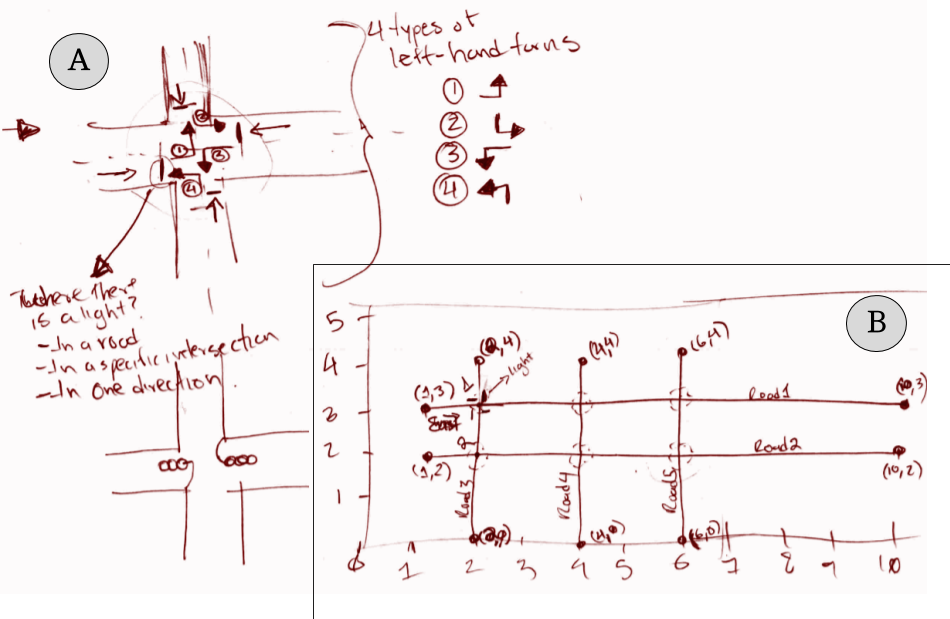
\includegraphics[width=\columnwidth]{figures/P4sketches}
\caption{External artifacts created by P1 during study; \protect\circled{A} shows a model of the interactions within a traffic intersection, \protect\circled{B} represents a potential layout for roads and intersections on a grid.}
\label{P4Sketch}
\end{figure}

%%%% ENTER SUNSET PARA

%We conclude from all our observations that along with the \textit{representational} and \textit{interactional} components of context, there exists an informational component. Participants looked for different types of information and consumed different amounts of information from various representations that have been known to affect context viz. time, environment etc. The various interactions determined how information was consumed by the participants. 